% Dokumentenklasse definieren.
\documentclass[
    12pt,
    a4paper,
    doubleside,
    BCOR=10mm,
    parskip=half,
    ngerman
]{scrbook}

% Die Header-Datei enthält alle verwendeten Pakete, sowie 
% Konfigurationen für Farben der Links und die Kopf- und 
% Fußzeilen. 
% Für den Druck kann "header.tex" in "header_print.tex" geändert werden, damit alle Verlinkungen und Markups schwarz bleiben.
\usepackage[utf8]{inputenc}
\usepackage[T1]{fontenc}

% Deutsches Sprachpaket für Babel auswählen
\usepackage[german] {babel}

% Font Änderungen
\usepackage{lmodern}
\usepackage[scaled]{helvet}
\renewcommand\familydefault{\sfdefault} 

% Integration von PDF Seiten. Wird zum Einfügen der eidesstattlichen Erklärung der Thesis verwendet.
\usepackage{pdfpages}

% Lipsum Fließtext generieren mit \lipsum 
\usepackage{lipsum}
\usepackage{cprotect}
\usepackage{csquotes}

% Kopf- und Fußzeilen der Seiten anpassen 
\usepackage{fancyhdr}

% Ersetzt \hline in Tabellen mit \toprule, \midrule und \bottomrule
\usepackage{booktabs}

% Unter anderem für mathematische Formeln
\usepackage{amsmath}

% Enthalten mathematische Symbole
\usepackage{amsfonts}
\usepackage{kpfonts}
\usepackage{amssymb}

% Generiert graphische Elemente, wie beispielsweise Diagramme
\usepackage{tikz}

% Bilder in Latex einbinden mit \includegraphics
\usepackage{graphicx}

% Den Pfad für alle Bilder relativ zur header.tex-Datei setzen.
\graphicspath{ {images/} }

% Tabellen automatisch an die Textbreite anpassen
\usepackage{tabularx}

% Mehrere Reihen in einer Tabelle zusammenschließen
\usepackage{multirow}

% Mehr Farben für LaTeX
\usepackage{xcolor}
\usepackage{color}
\definecolor{dkgreen}{rgb}{0,0.6,0}
\definecolor{dkblue}{rgb}{0,0,0.2}
\definecolor{gray}{rgb}{0.5,0.5,0.5}
\definecolor{mauve}{rgb}{0.58,0,0.82}
\definecolor{darkerred}{rgb}{0.2,0,0}

% Paket, um Links im Dokument zu erzeugen
\PassOptionsToPackage{hyphens}{url}\usepackage{hyperref}

% Farben und Art der Links anpassen
\hypersetup{
    colorlinks = true,
    linkcolor=black,
    filecolor=black,      
    urlcolor=black,
    citecolor=black
}

% Enumerationsliste mit römischen Zeichen
\renewcommand{\theenumi}{\roman{enumi}}
\usepackage{footnote}
\makesavenoteenv{figure}
\usepackage{epigraph}
\usepackage{listings}

% Umlaute in Listings zulassen
\lstset{literate=% Allow for German characters in lstlistings.
{Ö}{{\"O}}1
{Ä}{{\"A}}1
{Ü}{{\"U}}1
{ß}{{\ss}}2
{ü}{{\"u}}1
{ä}{{\"a}}1
{ö}{{\"o}}1
}

% Farben in Lstlistings verwenden
\lstset{frame=tb,
    language=Java,
    aboveskip=3mm,
    belowskip=3mm,
    showstringspaces=false,
    columns=flexible,
    basicstyle={\small\ttfamily},
    numbers=none,
    numberstyle=\tiny\color{black},
    keywordstyle=\color{black},
    commentstyle=\color{black},
    stringstyle=\color{black},
    breaklines=true,
    breakatwhitespace=true,
    tabsize=3
}

% Paket für Akronyme und Glossar
\usepackage[acronym,nonumberlist,order=letter,nopostdot,toc,numberedsection=autolabel,section=chapter]{glossaries}
%,style=super
\renewcommand*{\glspostdescription}{}
\setacronymstyle{long-short}

% Ändern der Farbe für Verlinkungen auf die Akronyme und in das Glossar auf ein dunkles Rot.
\renewcommand*{\glstextformat}[1]{\textcolor{black}{#1}}
\makenoidxglossaries{}

\usepackage[doublespacing]{setspace}
\usepackage{background}
\usepackage{lastpage}

% Mit dem Command \subautor kann jedem einzelnen Kapitel ein einzelner Autor hinzugefügt werden
\newcommand{\subautor}[1]{\begin{flushright}
    {\small\textit{#1}}    
\end{flushright}}

% Notwendig, um die Verlinkung in das Inhaltsverzeichnis über die Fußzeile zu erstellen.
\backgroundsetup{contents={}}

% Normaler Stil für Seiten innerhalb der Arbeit
\pagestyle{empty}
\renewcommand{\headrulewidth}{0pt}% removes header line
\lhead{\leftmark}
\rhead{}
\cfoot{\thepage}
\lfoot{\hyperlink{contents}{\small{Inhaltsverzeichnis}}}% links the TOC at the center of the page footer

% Am Ende der Arbeit werden die Kapitelreferenzen in der Kopfzeile entfernt.
\renewcommand{\headrulewidth}{0pt}% removes header line
\lhead{}
\rhead{}
\cfoot{\thepage}
\lfoot{}

% Am Anfang des Dokuments werden alle Kopf- und Fußzeilen entfernt.
\AtBeginDocument{\addtocontents{toc}{\protect\thispagestyle{empty}}}


% Das Glossar wird am Anfang erstellt. Wenn kein Glossar und keine Akronyme verwendet werden, die folgenden drei Zeile auskommentieren.
\loadglsentries{appendix/glossar.tex}
\loadglsentries{appendix/acronyms.tex}

\begin{document}
% Keinen Styline (Seitennummer, usw.) auf der Titelseite
\pagestyle{empty}
% Den Abstand zwischen den Zeilen leicht vergrößern, um die Lesbarkeit zu erhöhen
\setstretch{1.0}
% Einfügen der Titelseite in das Projekt. Der angegebene Pfad der eingefügten
% .tex-Datei ist relativ zu dieser Datei.
\begin{titlepage}
    % Kopfzeile enthält das INFLogo als Bild
    \begin{figure}
        \begin{flushright}
            
\includegraphics[scale=0.75]{images/INFLogo.png}
        \end{flushright}
    \end{figure}

    {\centering

    \vspace{4.5cm}
    {\Large Bachelorarbeit}\\
    (oder Seminar Ausgewählter Themen)\\
    \vspace{1.5cm}
    {\LARGE{\textbf{Hier steht der Titel Ihrer Bachelorarbeit}}}\\
    \vspace{2cm}

    \vspace{1.0cm}
    Erika Mustermann\\
    Matrikel-Nr.: 12345\\
    \vspace{2.0cm}
    Erstprüfer: Prof.\ Dr.\ Manuela Mustermann\\
    \vspace{0.5cm}
    ZweitprüferIn: Prof.\ Dr.-Ing.\ Max Mustermann\\
    \vspace{1.5cm}
    {\small Abgabedatum: 21.12.2030}\\
    \vspace{1.5cm}
}

    % Fußzeile enthält die Anschrift und das Logo der Reutlingen University
    \backgroundsetup{
      scale=1,
      color=black,
      opacity=1,
      angle=0,
      position=current page.south,
      vshift=60pt,
      hshift=-200pt,
      contents={%
      \begin{minipage}{.18\textwidth}
      
\includegraphics[width=1000pt,height=70pt,keepaspectratio]{images/FHRTFooter.png}
      \end{minipage}%
      }
    }
\end{titlepage}

{\small
\textbf{Abstract:}\\
Virtual Reality (VR) gilt als vielversprechende Technologie, die heutzutage nicht mehr
wegzudenken ist. Ein Grund dafür ist, dass es noch nie so einfach war, komplexe Inhalte mit
einem hohen Potenzial für Interaktivität zu vermitteln. Die Vorteile virtueller Trainings sind
vor allem die Schulungen bei gefährlicher Arbeit oder wenn diese kosten- und zeitaufwendig
sind. Deshalb wird in der in der Raumfahrt vermehrt das Training mit VR eingesetzt. Für die
geplanten neuen Missionen der NASA ist die Entwicklung neuer Trainings und der
zugehörigen VR- Technologien erforderlich. Dabei kann auf etliche vorhandene
Entwicklungen zurückgegriffen werden. Diese Literaturarbeit befasst sich mit den Systemen
Simplified Aid for EVA Rescue (SAFER) SAFER und Charlotte einem Mass Handling
System. Das Verständnis dieser Systeme kann helfen, zukünftige Systeme zu designen und
zu entwickeln
}
% Für die PDF Version den Link links unten auf der Seite auf das Inhaltsverzeichnis setzen
\hypertarget{contents}{}
% Automatisches Anlegen des Inhaltsverzeichnis
\tableofcontents

% Neue Seite nach dem Inhaltsverzeichnis einfügen
\newpage
% Neuen Stil für jede Seite, der Stil kann in der header.tex Datei geändert werden.
% Der Stil deklariert die Kopf- und Fußzeilen der folgenden Seite.
\pagestyle{fancy}

% Erstes Kapitel, die \chapter, \section, \subsection, usw. werden automatisch
% dem Inhaltsverzeichnis hinzugefügt
\chapter{Einführung}
Das Tutorial enthält verschiedene Sektionen zur Beschreibung grundlegender Funktionen in \LaTeX.\footnote{Vielen Dank an Ihren Kommilitonen Oliver Schneider, der diese Vorlage erstellt hat!}
Zuerst werden die \nameref{sec:basics} in Kapitel~\ref{sec:basics} beschrieben.
Dort sind die \nameref{sec:basics-text}, die \nameref{sec:basics-lists}
und das \nameref{sec:basics-contents} beschrieben.
Darauf folgend ist die Verwendung und Erstellung von \nameref{sec:BilderTabellenListings} in Kapitel~\ref{sec:BilderTabellenListings} erklärt.
Verwaltung und richtiges Zitieren in \LaTeX~ist im Kapitel~\ref{sec:bibliography} zu finden.
Die Verwendung von einem Glossar und Akronym-Verzeichnis ist im Kapitel~\ref{sec:glossary} enthalten.
Wichtige Quellen dieser Arbeit sind~\cite{Dermeval2015},\cite{pohl2016requirements}.

\LaTeX~kann auf nahezu allen Plattformen (Mac,Linux, Windows und Online) installiert werden.
Hierfür kann der Link in der Fußzeile aufgerufen werden.

Für die effiziente Bearbeitung Ihrer Arbeit empfehlen wir Texmaker\footnote{\url{https://www.xm1math.net/texmaker/}}.
Dafür brauchen Sie eine unterliegende LaTeX Installation, z.B.~die Tex-Live Installation\footnote{\url{http://tug.org/texlive/}}.
Meist reicht die Standardinstallation.
Wenn Sie die Tex-Dateien manuell kompilieren wollen, müssen Sie in einer Kommandozeile folgendes tun:
\begin{enumerate}
    \item Terminal öffnen und mit \lstinline|cd| in den Hauptordner des Projekts navigieren
    \item \lstinline|pdflatex tutorial.tex| eingeben und mit Eingabetaste bestätigen.
    \item \lstinline|makeglossaries tutorial| erstellt die Akronyme und das Glossar.
    \item Die Befehle \lstinline|bibtex tutorial| und  \lstinline|biber tutorial| Befehl erstellen das Literaturverzeichnis.
    \item Erneut \lstinline|pdflatex tutorial.tex| ausführen, um Akronyme, Glossar und das Literaturverzeichnis einzufügen.
\end{enumerate}


In \LaTeX kann man ein Wort mit \lstinline|\textbf{wort}| \textbf{fett} und mit
\lstinline|\textit{wort}| \textit{kursiv} schreiben.\\
\par
Ein Sprung in eine neue Zeile in einem \LaTeX Dokument wird nicht mit
der Eingabetaste, sondern mit den Zeichen \lstinline|\\| erreicht.\\
\\
\textbf{Beispiel:}\\
Nach diesem Satz wird eine neue Zeile begonnen.\\
Das ist die neue Zeile.\\
\par
Eine neuer Absatz ist mit dem Befehl \lstinline|\par| möglich.\\
\\
\textbf{Beispiel:}\\
Nach diesem Satz wird ein neuer Absatz entstehen.\\
\par
Dieser Satz steht in einem neuen Absatz.\\
\par
Nach dem Befehl \lstinline|\newpage| wird auf der Text auf der folgenden Seite fortgesetzt.\\
\\
\textbf{Beispiel:}\\
Der nächste Satz wird auf einer neuen Seite stehen.\\
\newpage
Dieser Satz steht auf einer neuen Seite.

\chapter{VR Training in der Raumfahrt}\label{sec:raumfahrt}

Dieses Kapitel beschäftigt sich mit Frage, wie VR Technologien für das Taining der Astronauten in der Raumfahrt eingesetzt wird.\\
Es geht im Speziellen um die Systeme Simplified Aid for EVA Rescue (SAFER) und ein Mass Handling System mit dem Spitzname Charlotte.
Bei diesen wird im Training der Astronauten VR- Technologie angewannt. Außerdem wird VR Training auch für Extra Vehicular
Activities (EVAs) eingesetzt.

\section{Einsatz bei SAFER}\label{sec:raumfahrt-safer}
Bei SAFER (Simplified Aid for EVA Rescue) handelt es sich um System, dass zur Selbstrettung verwendet wird. \cite{moore201021st}
Es ist während EVAs am Raumanzug befestigt und wird eingesetz, wenn ein Atronaut unabsichtlich von der ISS getrennt wird. \cite{miralles2013onboard}
SAFER besteht aus einem Triebwerksrucksack mit gasförmigem Stickstoff. \cite{moore201021st}
Es wird deshalb auch als "Jetpack" bezeichnet. \cite{garcia2020training}.
Der letzte Einsatz von SAFER liegt 30 Jahre zurück, trotzdem ist SAFER weiterhin für jeden EVA notwendig.\cite{garcia2020training}
\\
Die Simulation wird über ein VR Dead Mountet Display (HMD) dargestellt. \cite{garcia2020training}
Garcia et al. führen aus, dass beim erste VR Headset der Systems 2012 ein Laptop auf den Kopf des Astronauten geschnallt wurde.
Dadurch konnte die VR Technologie auch auf der ISS das erste Mal zum trainieren benutzt werden. \cite{garcia2020training}
2020 wurden dann laut Garcia et al. die Vive Pro HMDs eingesetzt. Dazu kommen noch Hand und Körpertracking sowie eine Handgestenerkennung. \cite{garcia2020training}
\\
Die SAFER Simulation beinhaltet die Physik-, Dynamik- und Sensordaten sowie Modelle für die Flugeigenschaften, Energie und Triebwerk. \cite{garcia2020training}
Simuliert werden kann eine Überprüfung des SAFER Systems, welche direkt vor einem EVA durchgeführt wird.
Der Ausbilder kann auf das Interface der Simulation zugreifen und kann Fehlermeldungen hervorrufen. Die Astronauten trainieren so, wie sie bei Fehlern reagieren müssen. \cite{garcia2020training}
Garcia et al. beschreiben noch eine zweite Einsatzmöglichkeit. Diese ermöglicht es, das SAFER system in VR zu fliegen. \cite{garcia2020training}
Laut Moore et al. wird beim Training ein Austronaut in der virtuellen Welt von der ISS getrennt und dieser muss sich selbst durch den Einsatz von SAFER retten. \cite{moore201021st}
Im Trainingsszenario taumelt der Astronaut 30 Sekunden von der ISS weg. Danach muss erfolgreich zurück zur ISS fliegen. Astronauten proben den Flug von SAFER viele Male mit unterschiedlichen Konfigurationen. Am Ende muss ein Prüfungsflug bestanden werden.
Auch an Bord der ISS hat der Austronaut dann nochmals die Möglichkeit zu trainieren. \cite{garcia2020training}
Ein Astronaut muss diese Technik der Selbstrettung gut beherrschen, da ihm sonst der Treibstoff ausgehen kann. \cite{moore201021st}

\section{Einsatz bei Charlotte}\label{sec:raumfahrt-charlotte}
Moore et al. beschreiben, dass die VR Trainingsstation für die akkurate Simulation des Umgangs mit schweren Bauteilen in der Schwerelosigkeit benutzt wird.\cite{moore201021st}
Charlotte besteht aus einem oder zwei Robotern. Dabei können zwei Astronauten gleichzeitig am selben Bauteil üben.\cite{miralles2013onboard}
Garcia et al. stellen in ihrer Arbeit die Trainingsstationen dar.
Die Trainingsumgebung ist so aufgebaut, dass zwei Astronauten sich Rücken an Rücken sitzen. Sie befinden gleichzeitig sich in einer verbundenen virtuellen Umgebung, bedienen aber zwei physische Charlotte Roboter.
Beide Astronauten tragen Vive Pro HMD, Handschuhe mit je einem Vive tracking Vorrichtung und einem Tracker für den Torso.
Die HMDs werden mit Windows PCs betrieben, die mit einer Nvidia 1080Ti Grphikkarte ausgestattet sind.
Außerdem läuft DOUG auf einem Linux Server Prozess. \cite{garcia2020training}
Mit Charlotte können Astronauten mit simulierten Bauteilen üben, die unterschiedlich schwer, groß und gewichtet sind. \cite{miralles2013onboard}
Charlotte wurde 1997 in das Training der Astronauten integriert und hat den Vorteil gegenüber früheren Traingsmethoden, das das Erscheinungsbild der Übungsmassen leicht verändert werden konnte. \cite{garcia2020training}
\\
Garcia et al. beschreiben , dass die auf der Interfaceplatte, Sensoren die vom Astronaut gewirkten Kräfte und Drehungen registriert.
Die Interfaceplatte ist die Schnittstelle zwischen Astronaut und simuliertem Bauteil, also die Griffe, die der Astronaut in der Hand hält.
Die DOUG Grafik wird dann auf dem HDM des Astronauten und dem Bildschirm des Ausbilders entsprechend geupdated. \cite{garcia2020training}
\\
Charlotte kann einfach verändert werden und kann dann andere pyhsikalische Bauteile simulieren.
Dabei müssen keine echten Gegenstände modelliert werden. \cite{garcia2020training}
Die Astronauten können solange mit Charlotte trainieren, bis sie sich mit dem Umgang von großen Massen in der Schwerelosigkeit wohl fühlen.\cite{garcia2020training}

\section{Einsatz bei EVAs}\label{sec:raumfahrt-eva}
Das Virtual Reality Labroratory ist eine der Trainingsstätten für das EVA Training am NASA Johnson Space Center(JSC). \cite{moore201021st}
Das VR LAb ist der einzige Ort, an dem Astronauten überall auf der ISS trainieren können, da es wegen der Größe der ISS keine echten Modelle gibt.
Die Mehrheit der durchgeführten VR Trainings beschäftigen sich mit EVAs.
Das VR Training wird hier zusätzlich zu anderen Methoden eingesetzt. \cite{osterlund2012virtual}
Osterlund et al. beschreiben weitere Vorteile des VR Trainings.
Durch die relative Position des Astronauten zur ISS und den zur Mission gehörenden Teilen können die Position des Piloten und des Roboterarmes korrigiert werden.
Dabei findet das Training in einer sicheren Umgebung statt. \cite{osterlund2012virtual}
\\
Moore et al. beschreiben, dass dort komplizierte EVAs am besten visualisiert und analysiert werden können. Außerdem kann das VR Training für Robotermanöver nur dort akkurat durchgeführt werden.
Die Austronauten studieren dort auch ihre Kommunikation und die Zeitliche Abfolge genau ein. \cite{moore201021st}
Miralles schreibt in ihrer Arbeit, dass Astronauten für verschiedene Arbeitsplätze auf der ISS üben können und sich damit vertraut machen können, welche Wege sie für EVAs nehmen sollten. \cite{miralles2013onboard}
Die eingesetzte Software heißt Dynamic Onboard Ubiquitious Graphics (DOUG). Sie kann auch an Bord der ISS genutzt werden, um bevorstehende EVAs zu trainieren. Dies macht die Astronauten selbstbewusster neue Techniken und Schritte anzuwenden. \cite{osterlund2012virtual}
Dies ist notwendig, da viele EVAs Reperatur Aufgaben geworden sind, die nicht vorher auf der Erde trainiert wurden.\cite{miralles2013onboard}
Osterlund et al. beschreiben DOUG als eine 3D Animation der ISS in der neuesten Konfiguration.
\\
Sie wird nicht nur für das Training, sondern auch in der Planung und beim Nachvollziehen der Arbeitsschritte eingesetzt.
Es handelt sich dabei um einen Prototypen, der eine billige Lösung darstellt.  \cite{osterlund2012virtual}
Das liegt daran, dass das System schnell angepasst weren kann und so eine Vielzahl von Szenarien evaluiert werden können.
DOUG kann für hochrealistische Trainingsszenarien eingesetzt werden. \cite{miralles2013onboard}
Astronauten können sich mit dem Arbeitplatz für das Space Station Remote Manipulator System (SSRMS) vertraut machen. Damit können Bauteile und Astronauten außerhalb der ISS bewegt werden.\cite{garcia2020training}
Miralles bescheibt, dass im VR Lab zusätzlich realistische Lichtverhältnisse simuliert werden.
Außerdem können Szenarien mit dem Einsatz des Roboterarmmes und zwei weiteren Astronauten trainiert werden. \cite{miralles2013onboard}
\\
Das Training für EVAs findet normalerweise Monate vor dem Flug zur ISS statt. Spezifische Aufgaben werden auf der Erde geplant und dann eine Gruppe von Astronauten speziell darauf trainiert. \cite{garcia2020training}
%\subsection{Unterkapitel}\label{sec:basics-subsection}
%\lipsum[1]


\chapter{Bilder, Tabellen und Listings}\label{sec:BilderTabellenListings}
\section{Bilder}
\subsection{Einfaches Bild volle Textbreite}\label{sec:images-textwidth}

\begin{figure}[!ht]
    \centering
    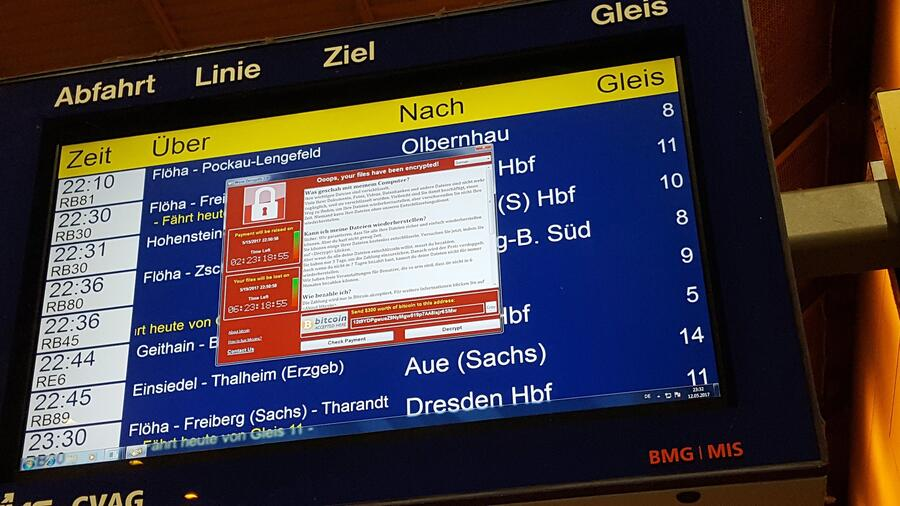
\includegraphics[width=1.0\textwidth]{images/example}
    \caption{\label{fig:example}Beispielbild\protect
    }
\end{figure}

In der Abbildung~\ref{fig:example} ist ein Beispielbild zu sehen.
Bilder werden mit \lstinline|\begin{figure}| eingeleitet.
Mit \lstinline|\includegraphics[width=1.0\textwidth]{Pfad/zum/Bild}| wird 
das Bild hinzugefügt, wobei das Bild durch die Zahl skaliert werden kann.
Das Pfad/zum/Bild ist mit dem relationalen Pfad zum Bild vom Projektordner aus zu ersetzen. 


\subsection{Mehrere Bilder nebeneinander}\label{sec:images-multiple}
\begin{figure}[!htb]
    \centering
    \hyperref[fig:big-example]{
    \minipage{0.46\textwidth}
        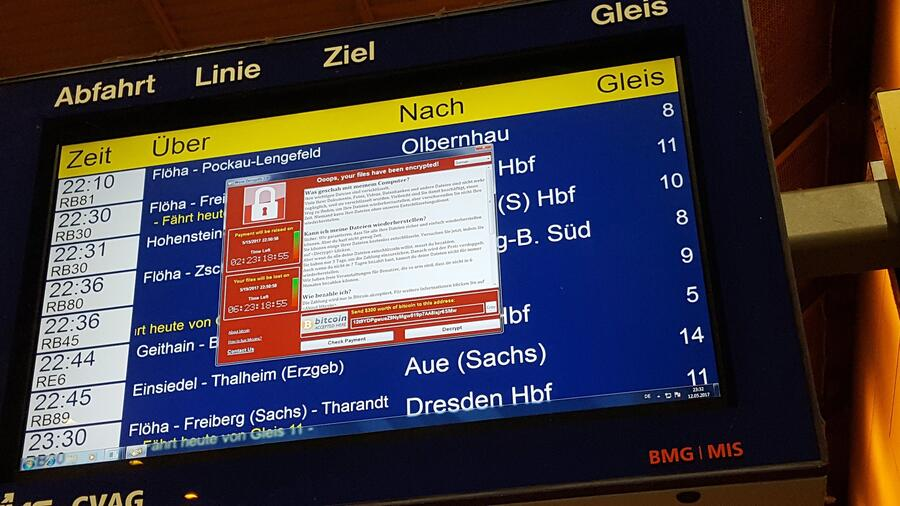
\includegraphics[width=\linewidth]{images/example}
        \caption{\label{fig:example-a}Beispielbild A}
    \endminipage\hfill
    }
    \hyperref[fig:big-example]{
    \minipage{0.46\textwidth}
        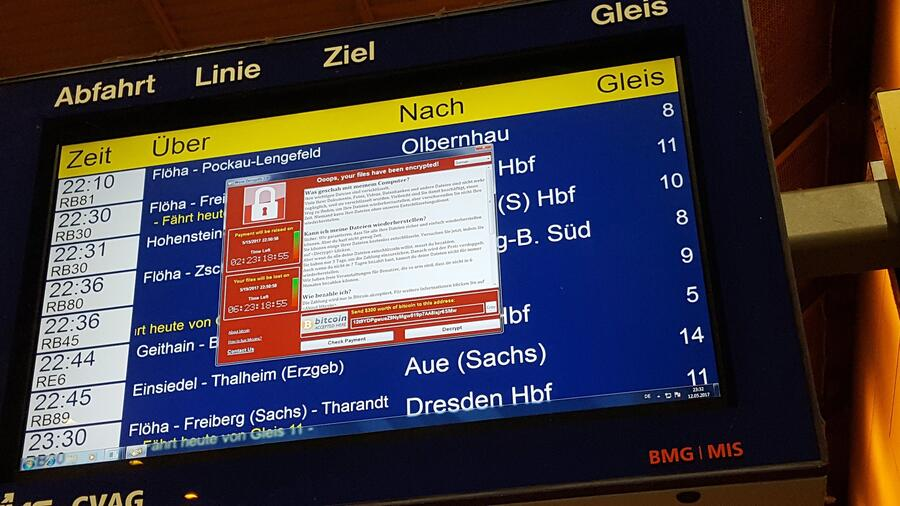
\includegraphics[width=\linewidth]{images/example}
        \caption{\label{fig:example-b}Beispielbild B}
    \endminipage\hfill
    }
    \hyperref[fig:big-example]{
    \minipage{0.46\textwidth}
        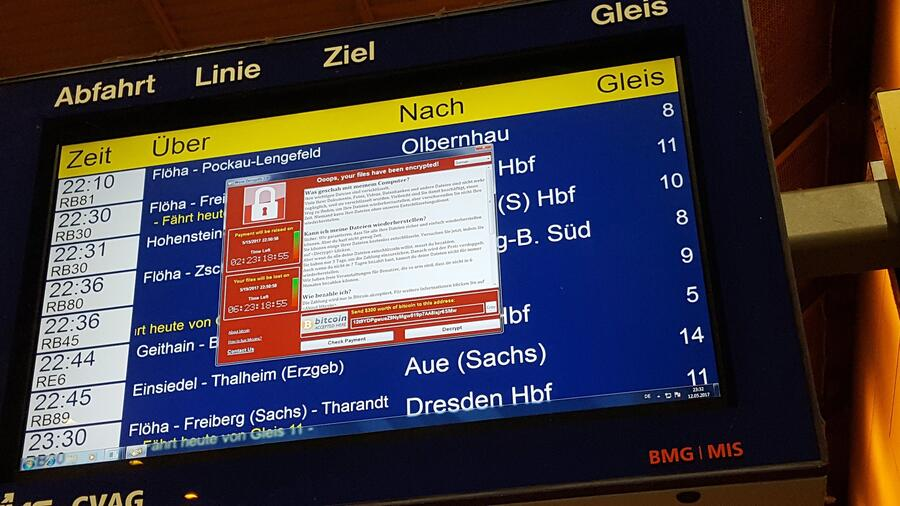
\includegraphics[width=\linewidth]{images/example}
        \caption{\label{fig:example-c}Beispielbild C}
    \endminipage\hfill
    }
    \hyperref[fig:big-example]{
    \minipage{0.46\textwidth}
        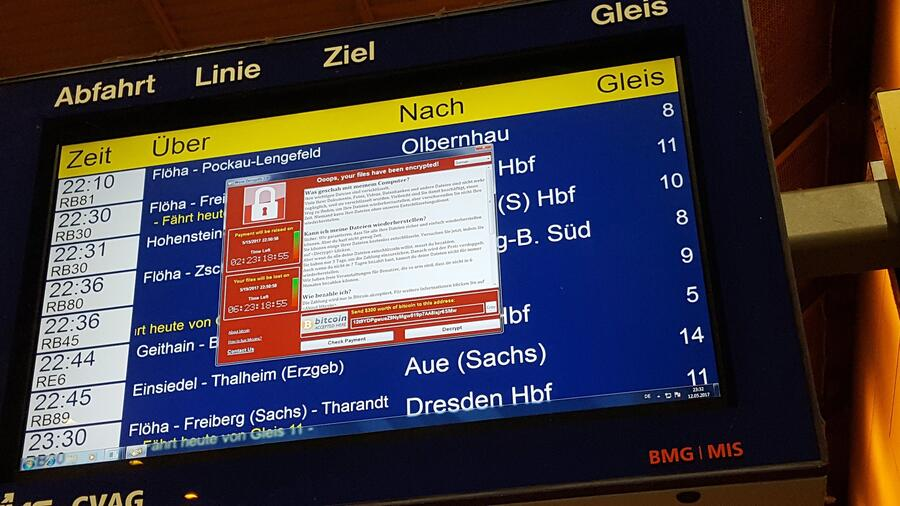
\includegraphics[width=\linewidth]{images/example}
        \caption{\label{fig:example-d}Beispielbild D}
    \endminipage\hfill
    }
    \caption{\label{fig:example-collection}Kollektion}
\end{figure}

In der \nameref{fig:example-collection} von Bildern in Abbildung~\ref{fig:example-collection}
ist die zusammenhängende Darstellung von Bildern gezeigt.
Die Bilder sind in den Anhang verlinkt. Wenn auf ein Bild geklickt wird, kann dieses 
in voller Größe im Anhang betrachtet werden.
Die Verlinkung ist in \path{attachments\bigpicture.tex} zu sehen.


\section{Tabellen}
\begin{table}[ht]
    \centering
    \begin{tabular}{ l c r }
        \toprule
                                & BIOS              & UEFI              \\
        \toprule
        \toprule
        Standardisiert          & Nein              & Ja                \\
        \midrule
        \midrule
        Aktualisierbar          & Nein              & Ja                \\
        \midrule
        \midrule
        Programmiersprache      & Assembler         & C                 \\
                                & schwer lesbar     & einfacher lesbar  \\
        \midrule
        \midrule
        Prozessormodus          & 16 Bit            & 32-64 Bit         \\
        Modulumsetzung          & Option-ROM        & Treiber           \\
        Parallele Ausführung    & Nein              & Ja                \\
        Geschwindigkeit         & Langsamer         & Schneller         \\
        \midrule
        \midrule
        \multicolumn{3}{l}{Verwendete Formatierung der Festplatten}\\
        \midrule
                                & MBR               & GPT               \\
                                & max 4 Partitionen & unlimitiert Partitionen\\
                                & max 2.1TB/HDD     & max 9.44ZB/HDD    \\
        \bottomrule
    \end{tabular}
    \caption{Vergleich von BIOS und UEFI}\label{tab:bios_uefi}
\end{table}

In Tabelle~\ref{tab:bios_uefi} ist ein Beispiel für eine Tabelle zu sehen.
Die Anzahl der Spalten wird nach \lstinline|\begin{tabular}| definiert.
Hier wird gleichzeitig auch die Textausrichtung mit c(=center),l(=left) oder r(=right) gesetzt werden. 
Die einzelnen Zellen der Tabelle werden mit \& voneinander getrennt und mit \lstinline|\\| beendet.
Mehrere Spalten können mit \lstinline|\multicolumn{x}{y}{Text}| verbunden werden,
wobei x die Anzahl der zusammengeführten Spalten und y die Textausrichtung (l, c oder r) ist.


\section{Listings}
\begin{lstlisting}[caption={HelloWorld Programm in Python},captionpos={b},label={lst:helloworld-python},language={Python}] 
    def main():
        print("Hello World\n");
        
    main()
\end{lstlisting}

Listings enthalten Quellcode von Programmen.
Das Beispiel in Listing~\ref{lst:helloworld-python} veranschaulicht das \nameref{lst:helloworld-python}.
Bei \lstinline|\begin{lstlisting}| sind in den eckigen Klammern folgende Eigenschaften definiert.
\begin{description}
    \item[caption] beinhaltet die Beschreibung des Listing
    \item[captionpos] positioniert die Beschreibung unter das Listing.
    \item[label] wird verwendet, um das Listing mit \lstinline|~\ref{lst:...}| im Text referenzieren zu können.
    \item[language] ist die Programmiersprache, die für das Markup verwendet wird.
\end{description}
Folgende Programmiersprachen sind im \lstinline|language|-Feld der Listings möglich.\\
ABAP2,4, ACSL, Ada4, Algol4, Ant, Assembler2,4, Awk4, bash, Basic2,4, C\#5, C++4, C4, Caml4, Clean, 
Cobol4, Comal, csh, Delphi, Eiffel, Elan, erlang, Euphoria, Fortran4, GCL, Go (golang), Gnuplot, Haskell, 
HTML, IDL4, inform, Java4, JVMIS, ksh, Lisp4, Logo, Lua2, make4, Mathematica1,4, Matlab, Mercury, MetaPost, 
Miranda, Mizar, ML, Modelica3, Modula-2, MuPAD, NASTRAN, Oberon-2, Objective C5 , OCL4, Octave, Oz, Pascal4, 
Perl, PHP, PL/I, Plasm, POV, Prolog, Promela, Python, R, Reduce, Rexx, RSL, Ruby, S4, SAS, Scilab, sh, SHELXL, 
Simula4, SQL, tcl4, TeX4, VBScript, Verilog, VHDL4, VRML4, XML, XSLT\footnote{Website mit unterstützten Programmiersprachen für Listings}. 


\chapter{Fazit}\label{sec:summary}
\section{Zusammenfassung}
Hier kommt die Zusammenfassung Ihrer Arbeit. 
Was haben Sie gemacht, welche Ergebnisse haben Sie erzielt. 

\section{Weitere Arbeiten}
Welche neue Ideen haben sich ergeben? 
Was müsste weiter untersucht werden? 
Welche weiteren Bachelor- oder Masterarbeiten sind in dem Themenfeld nun interessant geworden? 

\backmatter

\chapter{Glossar und Akronyme}\label{sec:glossary}
Die Beschreibung des Begriffs \gls{acronym} wird im Glossar erklärt.
Hierfür wird in der Datei \path{appendix/glossary.tex} der entsprechende Eintrag hinzugefügt.
Mit dem \lstinline|\gls{glossar-referenz}| Befehl kann man die Begriffe im Text auf direkt in das Glossar verlinken.\\
\par
\glspl{acronym} selbst wie beispielsweise \gls{rz}, werden beim ersten mal ausgeschrieben.
Wird \gls{rz} ein zweites Mal verwendet, ist nur die Abkürzung im Text zu sehen.
\glspl{acronym} werden in der Datei \path{attachments/acronyms.tex} definiert und 
können zur Definition des \gls{acronym}s in das Glossar weiter verlinkt werden.


% Für die Akronyme, die Literatur und das Glossar wird der Zeilenabstand reduziert.
\singlespacing{}
% Hier werden die Akronyme und das Glossar in das Dokument geschrieben
\printnoidxglossary[type=\acronymtype,title={Abkürzungen\label{akronyme}}]
% Glossaa
\printnoidxglossary[title={Glossar}]

% Hier wird das Literaturverzeichnis in das Dokument geschrieben
% Das Literaturverzeichnis bekommt keine Kapitelnummer im Inhaltsverzeichnis und wird mit einem * versehen
\newpage
\addcontentsline{toc}{chapter}{Literatur}
\bibliographystyle{alpha}
\bibliography{references}

\newpage
% Anhang erstellen, da dieser ebenfalls keine Nummerierung bekommt,
% wird wieder der Asterix (*) nach \chapter verwendet.
\chapter{Anhang}\label{appendix}
\section{Zusätzliche Informationen}\label{att:bigpicture}
Im Anhang platzieren Sie weitere Informationen aus dem Kontext Ihrer Arbeit.
Wichtige Ergebnisse, die Sie erzielt haben, gehören allerdings nicht hierher.
\end{document}
